\section{Power/fifth chords}

The power chord, or more formally called a fifth chord, is a chord where you only play the root and the perfect 5th.

Power chords don't have the 3rd, meaning that they are neither major of minor.

Power chords are often used on electric guitar with distortion. If you would play the full chord (with the 3rd), it can sound quite muddy depending on the amount of distortion.

% https://www.hooktheory.com/blog/power-chords/

\subsection{Notation}
A power chord can be indicated by (taking the C chord as an example):

\begin{itemize}
	\item C5
	\item C(no 3)
\end{itemize}

Both indicate that the chord doesn't contain the 3rd.

\subsection{Example}

\begin{figure}[h]
	\centering
	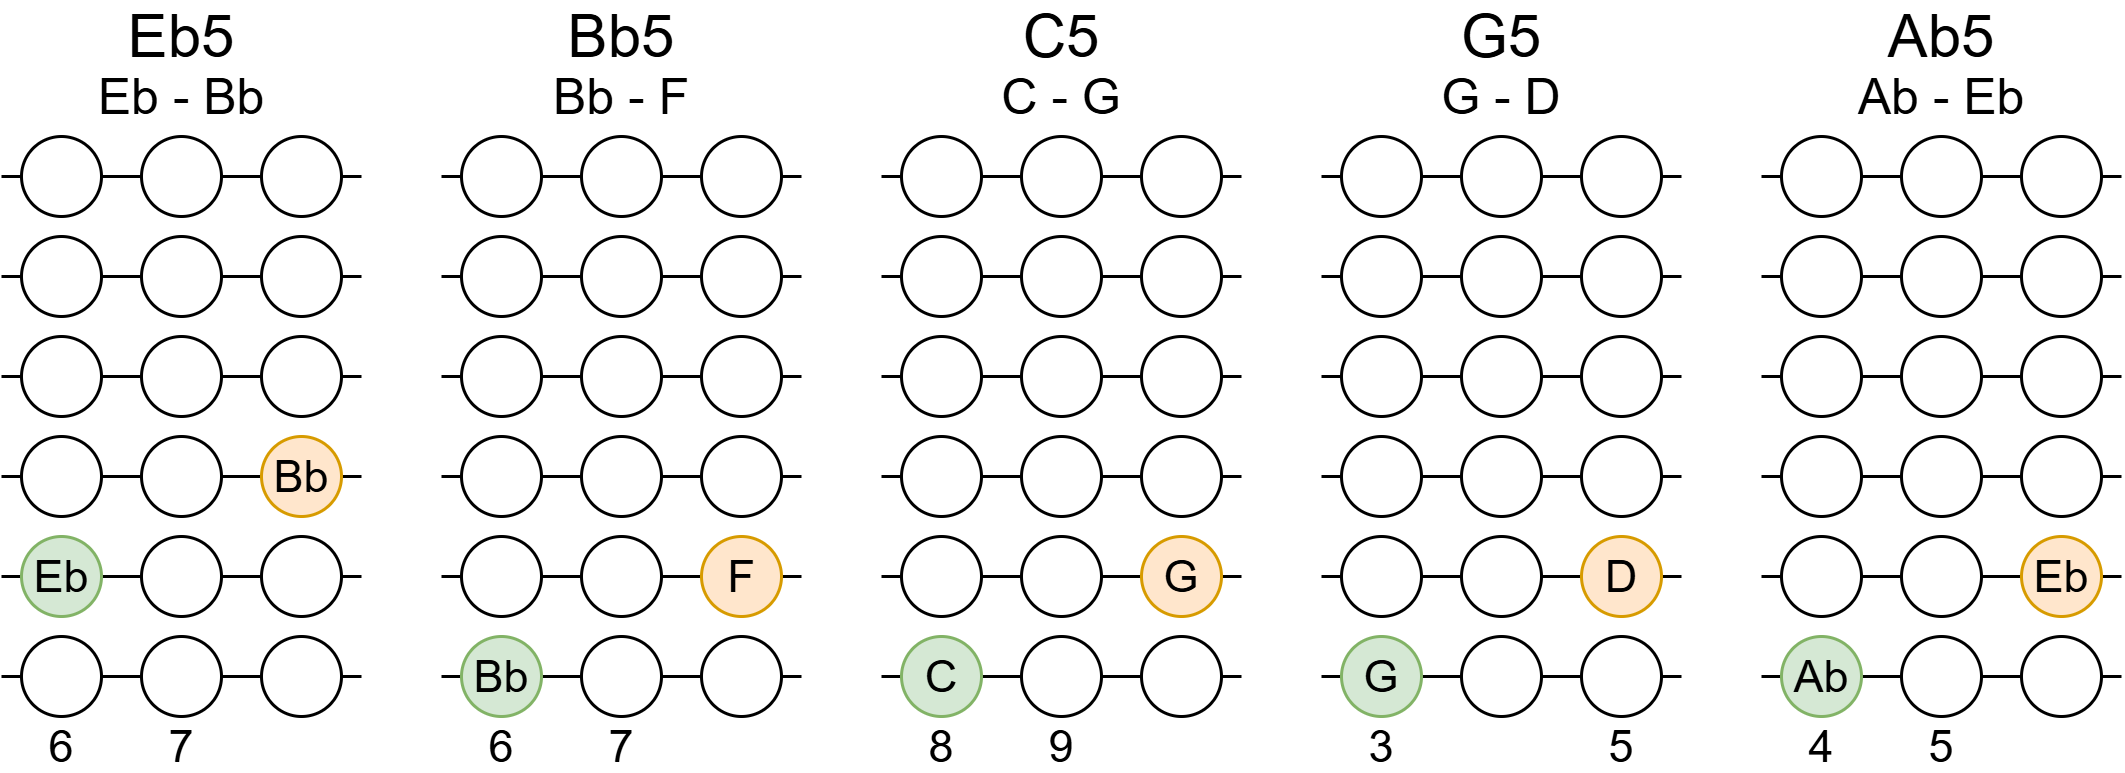
\includegraphics[height=0.16\textheight]{../../Images/ChordsUsedInBasketCaseGreenDayVerse1.png}
	\caption{Chords used in verse 1 of "Basket Case - Green Day"}
	\label{fig:guitar_chords_verse_1_basket_case_green_day}
\end{figure}

Note that on most places on the internet you will find just the chord names without the "5" or "(no 3)". In those cases you have to listen to the song to know what kind of chord is being played. In most cases, for punk, rock, metal, etc. kind of songs, powers chords are a safe bet.

\begin{song}[verse/numbered, align-chords=l]{title={Basket Case - Green Day (verse 1)}, music={Green Day}}
	\begin{verse}
		^{E$\flat$5}Do you have the ^{B$\flat$5}time to ^{C5}listen to me ^{G5}whine? \\
		^{A$\flat$5}About nothing and ^{E$\flat$5}everything, all ^{B$\flat$5}at once \\
		^{E$\flat$5}I am one of ^{B$\flat$5}those ^{C5}melodramatic ^{G5}fools \\
		^{A$\flat$5}Neurotic to the ^{E$\flat$5}bone, no doubt about ^{B$\flat$5}it \\
	\end{verse}
\end{song}

\newpage

\section{Chord inversions \& open/closed voicing}

So far we have learned that a basic chord consists of the \textbf{1st/root}, \textbf{3rd}, and \textbf{5th} degree of a (major or minor) scale stacked on top of each other.

Lets assume that we play all three notes\textbf{ within a single octave} (meaning that the 1st, 3rd, and 5th degree pitches are ascending). This means that the voicing of this chord is \textbf{closed} due to it being within a single octave.

\autoref{fig:c_major_inversions} shows the 1st inversion (C/E) and 2nd inversion (C/G). The 1st inversion means to play the 3rd degree (E) as the bass note. The 2nd inversion means to play the 5th degree (G) as the bass note. To keep the chord in a closed voicing (within a single octave), you simply move the current bass note one octave higher so that it now is the highest pitch in the chord.


\begin{figure}[h]
	\centering
	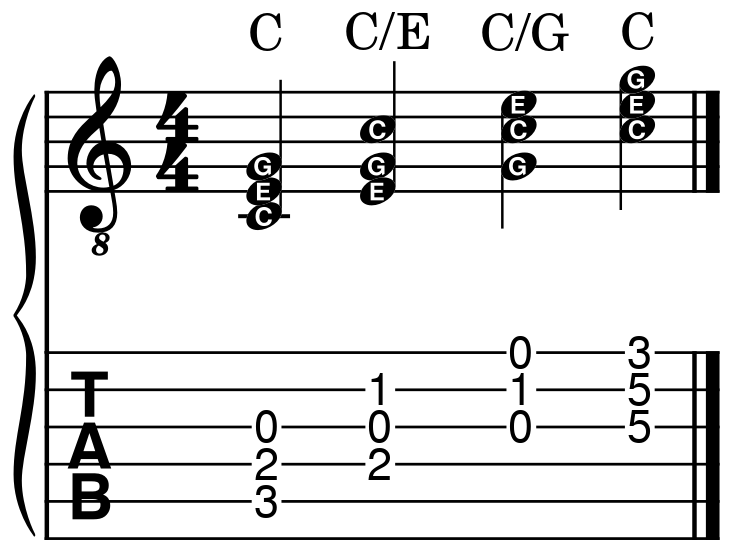
\includegraphics[height=0.13\textheight]{../../MuseScore/Guitar/CMajorInversions.png}
	\caption{Inversions of the C major chord/triad on guitar}
	\label{fig:c_major_inversions}
\end{figure}

Examples of open voicing (playing notes over 2 or more octaves) can be seen in \autoref{fig:c_major_open_voicings}.

\begin{figure}[h]
	\centering
	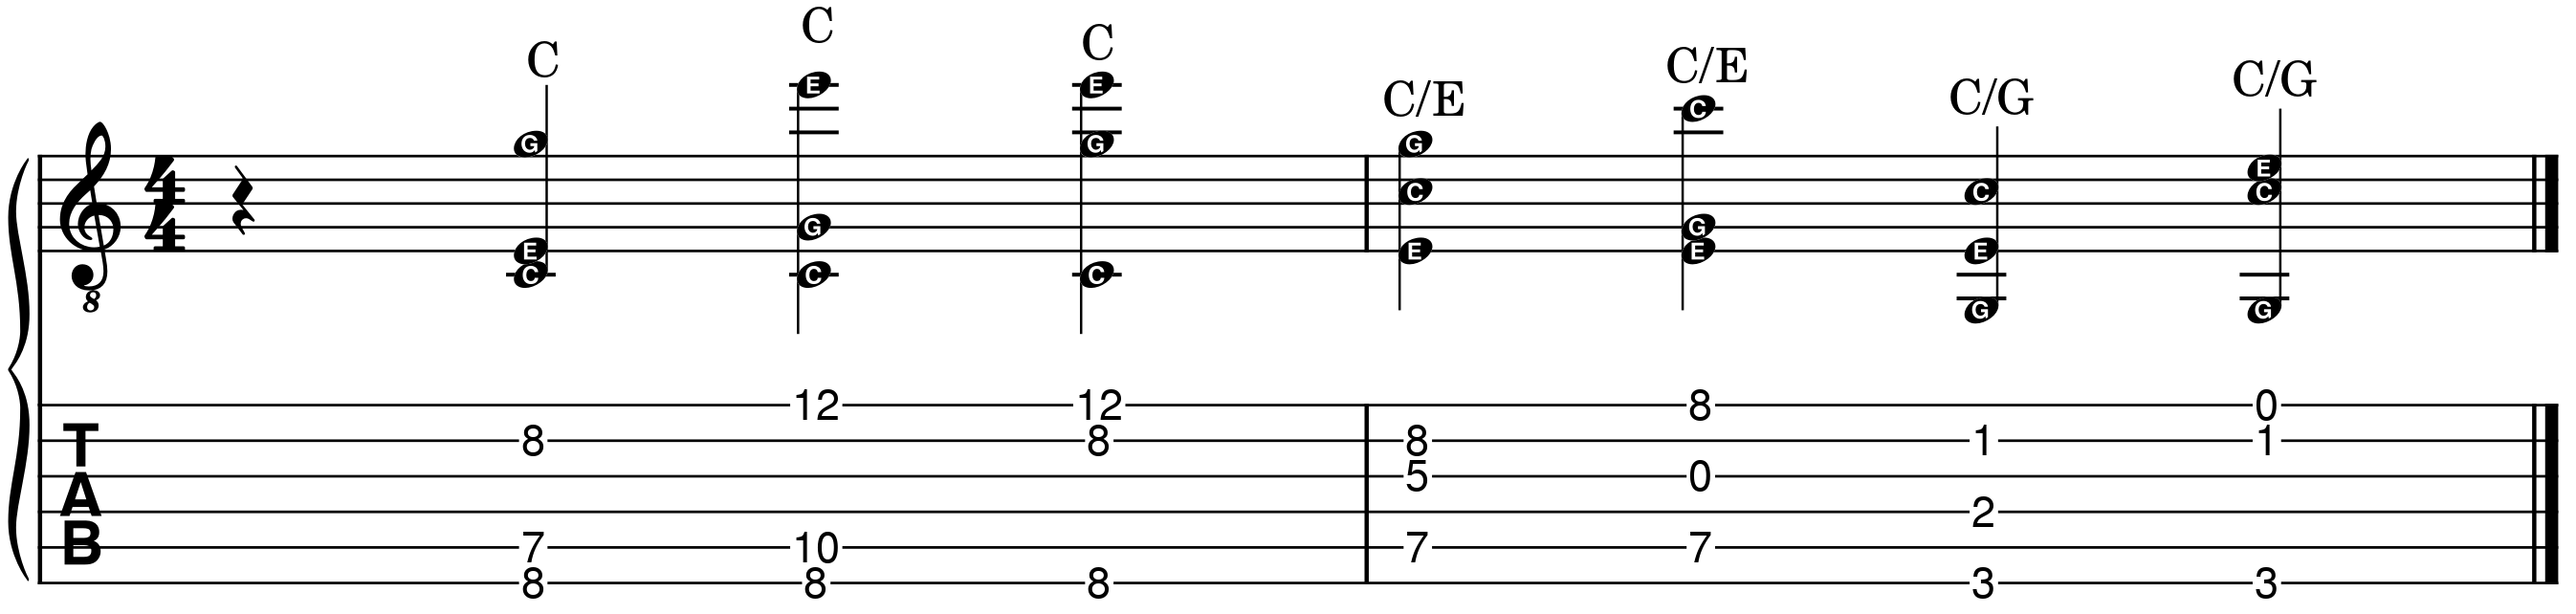
\includegraphics[height=0.13\textheight]{../../MuseScore/Guitar/CMajorOpenVoicings.png}
	\caption{Examples of open voicings for the C major chord}
	\label{fig:c_major_open_voicings}
\end{figure}

\newpage

\subsection{Examples}

In a previous section it was already shown that "We Are The Champions" from "Queen" uses chord inversions.

Another example is from Ed Sheeran's "Thinking out loud". Here the D 1st inversion (D/F\sharp) is played. The chord shapes are shown in \autoref{fig:guitar_chords_verse_1_thinking_out_loud_ed_sheeran}.

\begin{figure}[h]
	\centering
	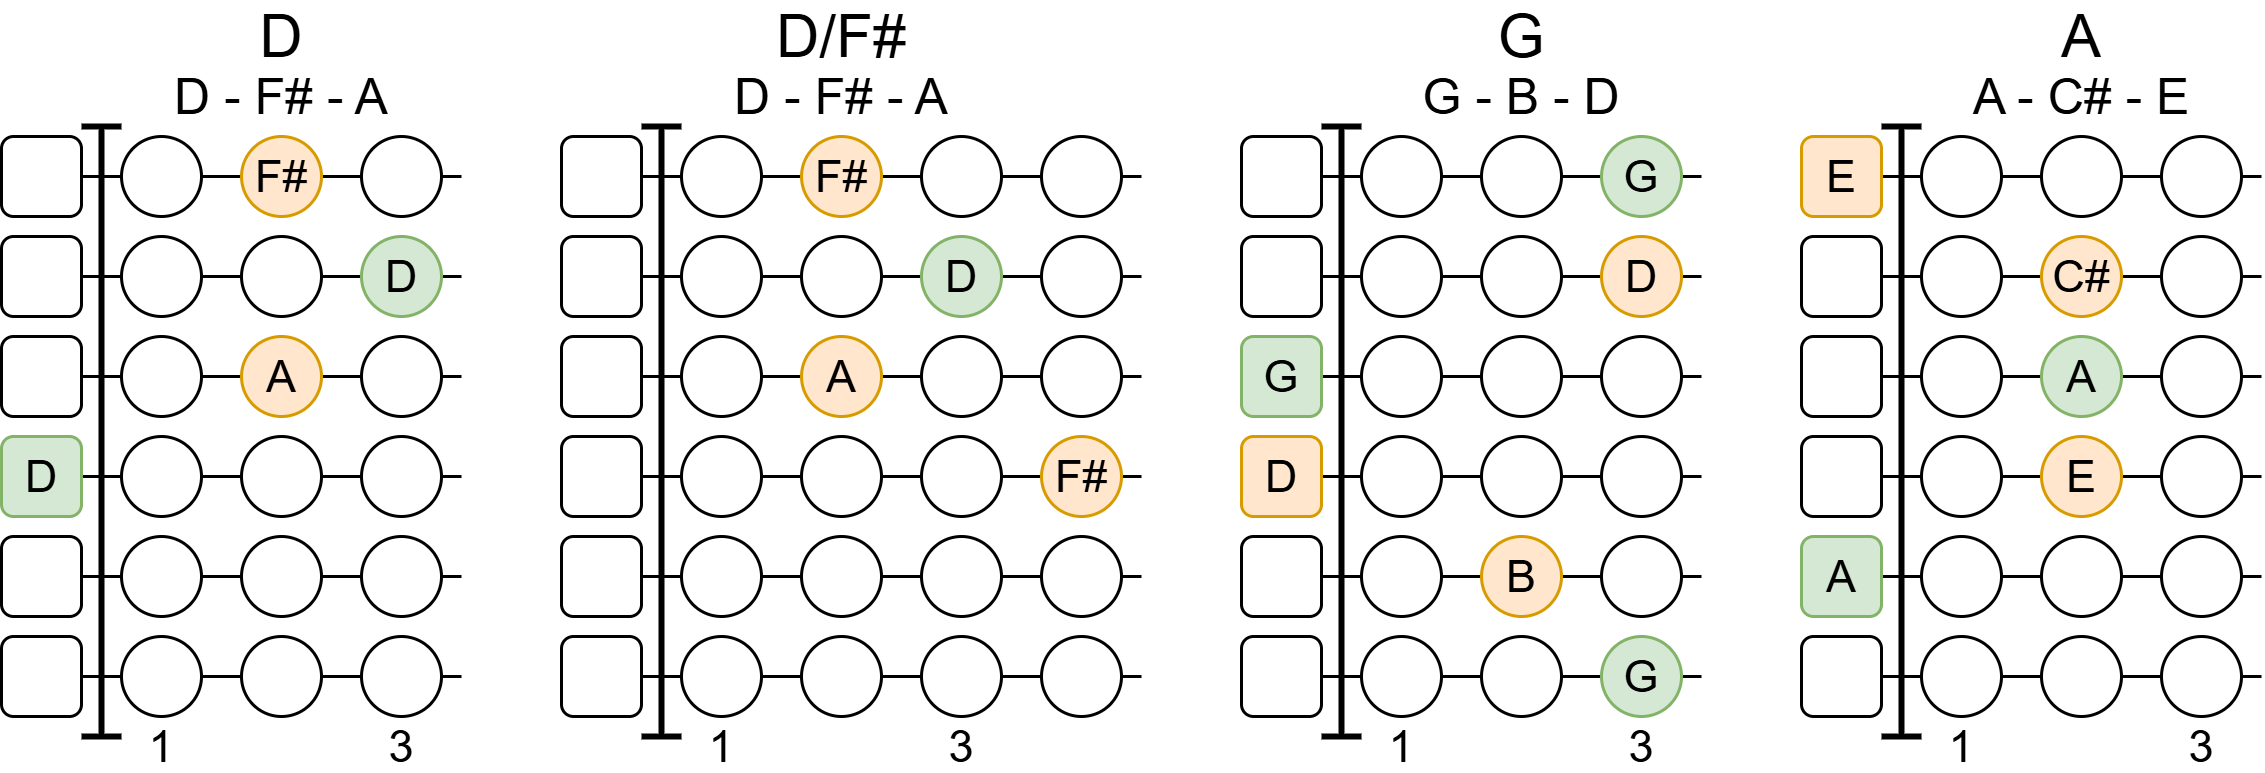
\includegraphics[height=0.16\textheight]{../../Images/EdSheeranThinkingOutLoudVerseChords.png}
	\caption{Chords used in verse 1 of "Thinking Out Loud - Ed Sheeran"}
	\label{fig:guitar_chords_verse_1_thinking_out_loud_ed_sheeran}
\end{figure}


\begin{song}[verse/numbered, align-chords=l]{title={Thinking out loud - Ed Sheeran (verse 1)}, music={Ed Sheeran}}
	\begin{verse}
		^{D} ^{D/F#}When your legs don't work like they ^{G}used to before ^{A} ^{D} \\
		^{D/F#}And I can't sweep you off of your ^{G}feet ^{A} ^{D} \\
		^{D/F#}Will your mouth still remember the ^{G}taste of my love ^{A} ^{D} \\
		^{D/F#}Will your eyes still smile from your ^{G}cheeks ^{A} \\
	\end{verse}
\end{song}

% Cadential 6 - 4

\newpage

\section{Diminished \& augmented chords}

Diminished and augmented chords have sort of an uneasy tone. This makes them great as a passing chord to bring in some tension.

Where major and minor chords are identified by their 3rd note, diminished and augmented chords are identified by their 5th note.

Simply put:

\begin{itemize}
	\item \textbf{Diminished} chord: \textbf{minor} chord with the \textbf{5th lowered} by a half step (1 semitone)
	\item \textbf{Augmented} chord: \textbf{major} chord with the \textbf{5th raised} by a half step (1 semitone)
\end{itemize}

\autoref{tab:guitar_diminished_intervals} and \autoref{tab:guitar_augmented_intervals} show how these relate to the major and minor scales (and chords created from them).

\begin{table}[h]
	\centering
	\begin{NiceTabular}{*{17}{c}}
		\Block{}{} & \Block{}{} & \Block{1-2}{\large{W}} & & \Block{1-2}{\large{H}} & & \Block{1-2}{\large{W}} & & \Block{1-2}{\large{W}} & & \Block{1-2}{\large{H}} & & \Block{1-2}{\large{W}} & & \Block{1-2}{\large{W}} & & \Block{}{} \\
		\Block{}{Minor intervals} & \Block[fill=ColorRootNote]{1-2}{1} & & \Block{1-2}{2} & & \Block[fill=ColorOtherNote]{1-2}{3$\flat$} & & \Block{1-2}{4} & & \Block[fill=ColorOtherNote]{1-2}{5} & & \Block{1-2}{6$\flat$} & & \Block{1-2}{7$\flat$} & & \Block{1-2}{8} & \\
		\Block{}{Diminished chord from minor scale} & \Block[fill=ColorRootNote]{1-2}{1} & & \Block{1-2}{} & & \Block[fill=ColorOtherNote]{1-2}{3$\flat$} & & \Block{}{} & \Block[fill=ColorOtherNote]{1-2}{5$\flat$} & & \Block{}{} & \Block{1-2}{} & & \Block{1-2}{} & & \Block{1-2}{} &
	\end{NiceTabular}
	\caption{Diminished intervals}
	\label{tab:guitar_diminished_intervals}
\end{table}

\begin{table}[h]
	\centering
	\begin{NiceTabular}{*{17}{c}}
		\Block{}{} & \Block{}{} & \Block{1-2}{\large{W}} & & \Block{1-2}{\large{W}} & & \Block{1-2}{\large{H}} & & \Block{1-2}{\large{W}} & & \Block{1-2}{\large{W}} & & \Block{1-2}{\large{W}} & & \Block{1-2}{\large{H}} & & \Block{}{} \\
		\Block{}{Major intervals} & \Block[fill=ColorRootNote]{1-2}{1} & & \Block{1-2}{2} & & \Block[fill=ColorOtherNote]{1-2}{3} & & \Block{1-2}{4} & & \Block[fill=ColorOtherNote]{1-2}{5} & & \Block{1-2}{6} & & \Block{1-2}{7} & & \Block{1-2}{8} & \\
		\Block{}{Augmented chord from major scale} & \Block[fill=ColorRootNote]{1-2}{1} & & \Block{1-2}{} & & \Block[fill=ColorOtherNote]{1-2}{3} & & \Block{1-2}{} & & \Block{}{} & \Block[fill=ColorOtherNote]{1-2}{5$\sharp$} & & \Block{}{} & \Block{1-2}{} & & \Block{1-2}{} &
	\end{NiceTabular}
	\caption{Augmented intervals}
	\label{tab:guitar_augmented_intervals}
\end{table}

In \autoref{sec:building_chords_with_diatonic_scale} you have already learned the following:

\begin{minipage}{0.5\textwidth}
	\begin{itemize}
		\item Minor chord: 1 - 3$\flat$ - 5:
			\subitem Interval 1 - 3$\flat$: minor 3rd
			\subitem Interval 3$\flat$ - 5: major 3rd
	\end{itemize}
\end{minipage}
\hfill
\begin{minipage}{0.5\textwidth}
	\begin{itemize}
		\item Major chord: 1 - 3 - 5:
			\subitem Interval 1 - 3: major 3rd
			\subitem Interval 3 - 5: minor 3rd
	\end{itemize}
\end{minipage}

Note that both the major and minor chords have a major and minor 3rd stacked on top of each other. Diminished chords have only minor thirds stacked and augmented chords have only major thirds stacked:

\begin{minipage}{0.5\textwidth}
	\begin{itemize}
		\item Diminished chord: 1 - 3$\flat$ - 5$\flat$:
			\subitem Interval 1 - 3$\flat$: minor 3rd
			\subitem Interval 3$\flat$ - 5$\flat$: minor 3rd
	\end{itemize}
\end{minipage}
\hfill
\begin{minipage}{0.5\textwidth}
	\begin{itemize}
		\item Augmented chord: 1 - 3 - 5$\sharp$:
			\subitem Interval 1 - 3: major 3rd
			\subitem Interval 3 - 5$\sharp$: major 3rd
	\end{itemize}
\end{minipage}

Earlier in this book at \autoref{sec:identifying_dimished_chords_in_the_scale} it was explained that a dimished chord has a tritone (meaning 6 semitones). This is the result of stacking two minor 3rd intervals.

% TODO: inversions

\subsection{Notation}
\begin{minipage}{0.4\textwidth}
	Diminished chords can be indicated by (taking C and the base):
	
	\begin{itemize}
		\item Cdim
		\item C($\flat$5)
		\item C\textsuperscript{o}
	\end{itemize}
\end{minipage}
\hfill
\begin{minipage}{0.4\textwidth}
	Augmented chords can be indicated by (taking C and the base):
	
	\begin{itemize}
		\item Caug
		\item C($\sharp$5)
		\item C+
	\end{itemize}
\end{minipage}

\newpage

\subsection{Examples}

% Diminished allstart + don't look back in anger - oasis

The song "All Stars" by "Smash Mouth" uses the diminished chord to bring in some tension (\autoref{fig:guitar_chords_in_all_stars_smash_mouth}).
 
\begin{figure}[h]
	\centering
	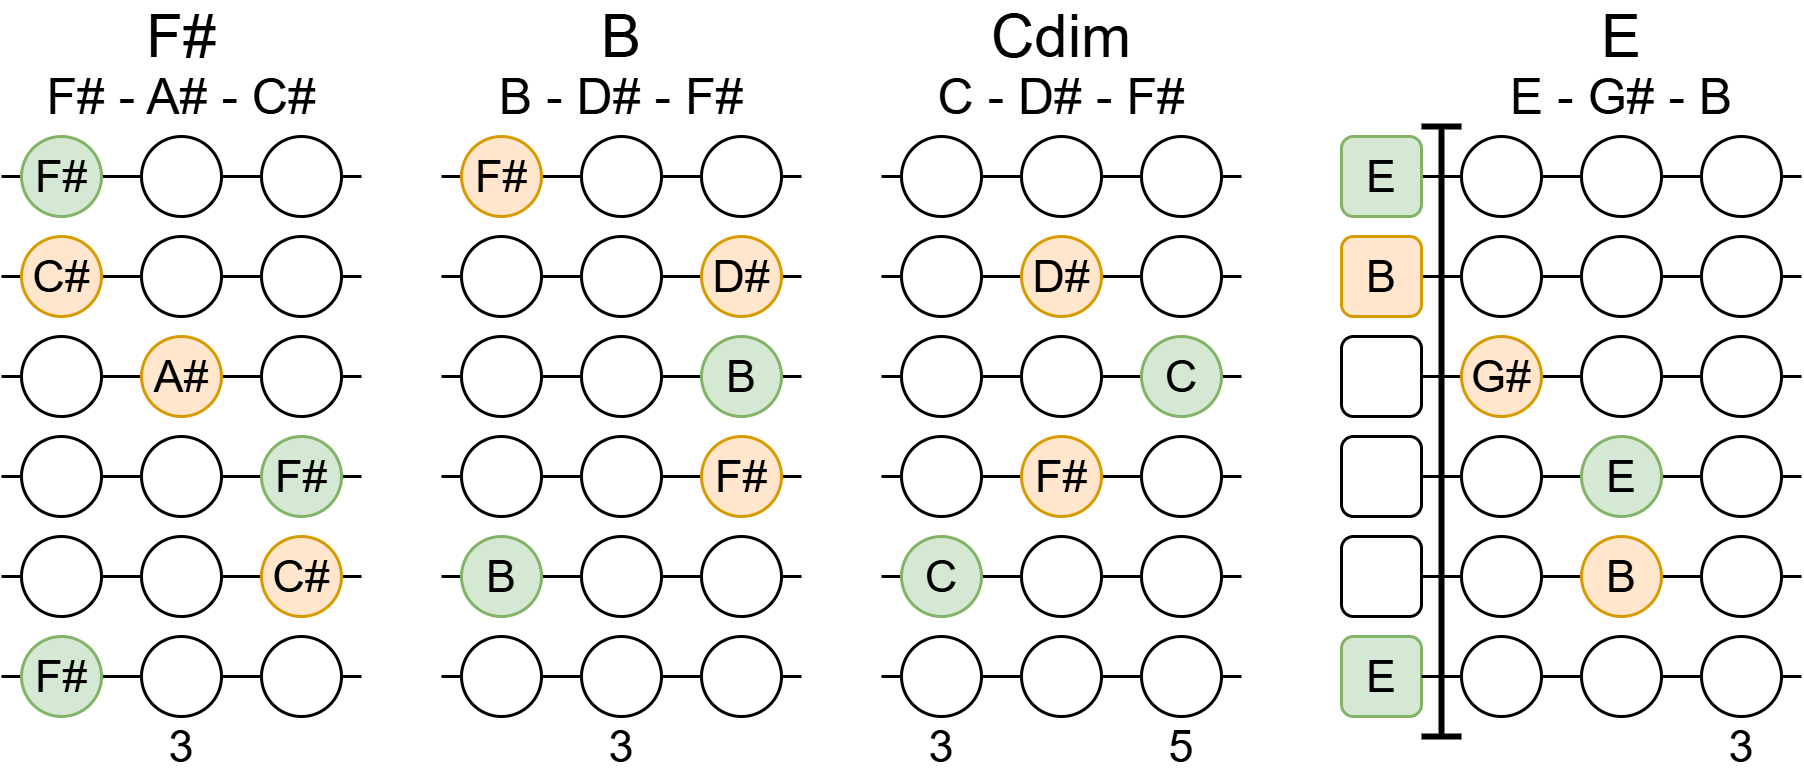
\includegraphics[height=0.16\textheight]{../../Images/ChordsInChorusAllStarsSmashMouth.png}
	\caption{Chords used in the chorus of "All Stars" by "Smash Mouth"}
	\label{fig:guitar_chords_in_all_stars_smash_mouth}
\end{figure}

\begin{song}[verse/numbered, align-chords=l]{title={All Stars - Smash Mouth (chorus)}, music={Smash Mouth}}
	\begin{chorus}
		^{F#}Hey now you're an ^{B}All Star get your ^{Cdim}game on, go ^{B}play \\
		^{F#}Hey now you're a ^{B}Rock Star get the ^{Cdim}show on get ^{B}paid \\
		And ^{F#}all that ^{B}glitters is ^{Cdim}gold \\
	 	^{B}Only shooting ^{F#}stars ^{E}break the ^{B}mold \\
	\end{chorus}
\end{song}


% Augmented Impossible Year Chords by Panic! At the Disco
% Augmented Stairway to heaven
% Augmented Life on mars - david bowie

The song "Impossible Year" by "Panic! At The Disco" uses augmented chords to create what is called a "line cliché". This is when either the root or the 5th of a chord is moved up (or down) a semitone a couple of times while keeping the rest of the notes the same. You see that happening here with the 5th of the F chord (see \autoref{fig:guitar_chords_used_in_impossible_year_panic_at_the_disco}).

\begin{figure}[h]
	\centering
	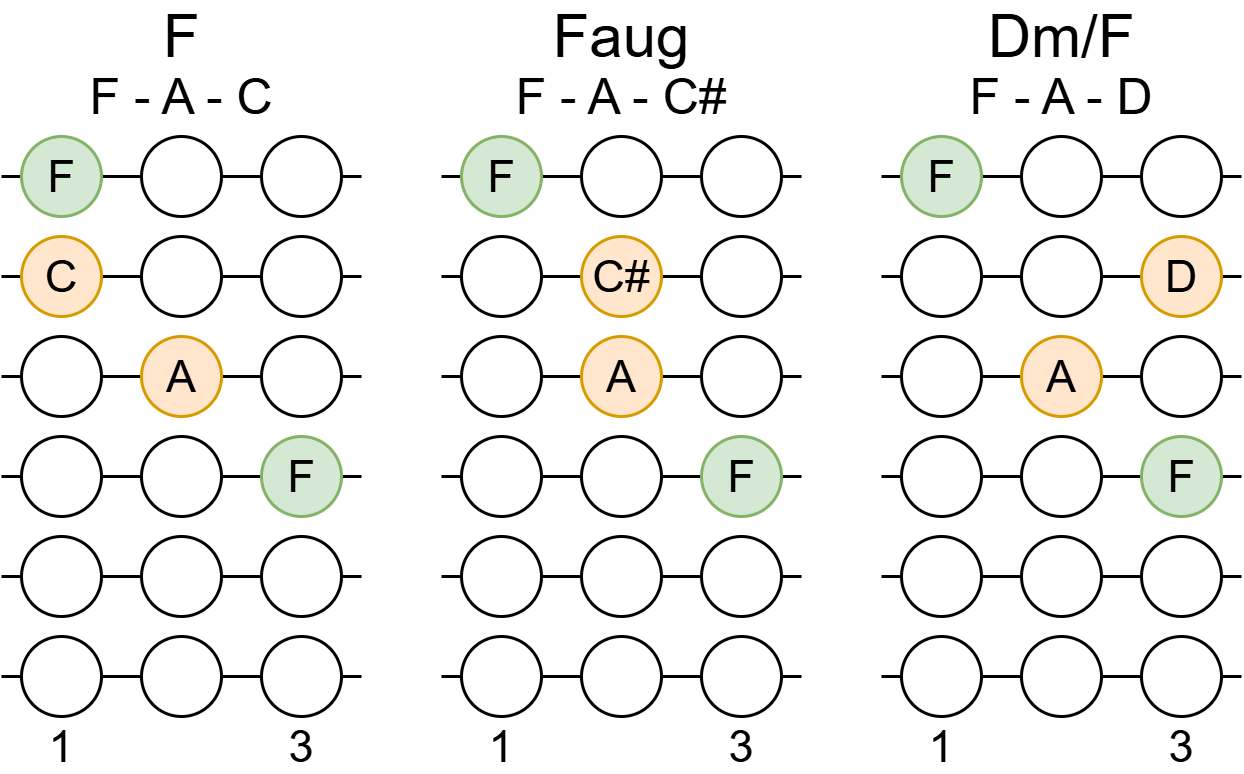
\includegraphics[height=0.16\textheight]{../../Images/ChordsUsedInImpossibleYearPanicAtTheDisco.png}
	\caption{Some of the chords used in "Impossible Year - Panic! At The Disco"}
	\label{fig:guitar_chords_used_in_impossible_year_panic_at_the_disco}
\end{figure}

\begin{song}[verse/numbered, align-chords=l]{title={Impossible Year - Panic! At The Disco (Part of Verse 1)}, music={Panic! At The Disco}}
	\begin{chorus}
		^{F}There's no sunshine ^{Faug} \\
		This ^{Dm/F}impossible year ^{Faug} \\
	\end{chorus}
\end{song}

\newpage

\section{7th chords}

First a reminder which chords in the major and minor scales are major, minor, and diminished.

\begin{table}[h]
	\begin{minipage}{0.45\textwidth}
		\centering
		\begin{NiceTabular}{*{16}{P{0.05mm}}}
			\Block{}{} & \Block{1-2}{\large{W}} & & \Block{1-2}{\large{W}} & & \Block{1-2}{\large{H}} & & \Block{1-2}{\large{W}} & & \Block{1-2}{\large{W}} & & \Block{1-2}{\large{W}} & & \Block{1-2}{\large{H}} & & \Block{}{} \\
			\Block{1-2}{1} & & \Block{1-2}{2} & & \Block{1-2}{3} & & \Block{1-2}{4} & & \Block{1-2}{5} & & \Block{1-2}{6} & & \Block{1-2}{7} & & \Block{1-2}{8} & \\
			\Block{1-2}{\RomanNumeralCaps{1}} & & \Block{1-2}{\RomanNumeral{2}} & & \Block{1-2}{\RomanNumeral{3}} & & \Block{1-2}{\RomanNumeralCaps{4}} & & \Block{1-2}{\RomanNumeralCaps{5}} & & \Block{1-2}{\RomanNumeral{6}} & & \Block{1-2}{\RomanNumeral{7}\textsuperscript{o}} & &
		\end{NiceTabular}
		\caption{Chords in the major scale}
		\label{tab:guitar_major_scale_chords_sec_7th_chords}
	\end{minipage}
	\hfill
	\begin{minipage}{0.45\textwidth}
		\centering
		\begin{NiceTabular}{*{16}{P{0.05mm}}}
			\Block{}{} & \Block{1-2}{\large{W}} & & \Block{1-2}{\large{H}} & & \Block{1-2}{\large{W}} & & \Block{1-2}{\large{W}} & & \Block{1-2}{\large{H}} & & \Block{1-2}{\large{W}} & & \Block{1-2}{\large{W}} & & \Block{}{} \\
			\Block{1-2}{1} & & \Block{1-2}{2} & & \Block{1-2}{3$\flat$} & & \Block{1-2}{4} & & \Block{1-2}{5} & & \Block{1-2}{6$\flat$} & & \Block{1-2}{7$\flat$} & & \Block{1-2}{8} & \\
			\Block{1-2}{\RomanNumeral{1}} & & \Block{1-2}{\RomanNumeral{2}\textsuperscript{o}} & & \Block{1-2}{\RomanNumeralCaps{3}} & & \Block{1-2}{\RomanNumeral{4}} & & \Block{1-2}{\RomanNumeral{5}} & & \Block{1-2}{\RomanNumeralCaps{6}} & & \Block{1-2}{\RomanNumeralCaps{7}} & &
		\end{NiceTabular}
		\caption{Chords in the minor scale}
		\label{tab:guitar_minor_scale_chords_sec_7th_chords}
	\end{minipage}
\end{table}

Now for each chord, we add the note that is two scale degrees up from the 5th degree to the chord/triad.

\subsection{Major and minor 7th chords}

An example for the root chord of the scale is shown in \autoref{tab:guitar_major_7th_chord_buildup} and \autoref{tab:guitar_minor_7th_chord_buildup}.

\begin{minipage}{0.43\textwidth}
	In \autoref{tab:guitar_major_7th_chord_buildup} (the major chord) a major 3rd (4 semitones) is stacked on the 5th degree. This results in a major 7 interval from the root note. This type of chord (a major chord with a major 7) is notated as a \textbf{M7} or \textbf{maj7} chord. For example, \textbf{CM7} or \textbf{Cmaj7}.
\end{minipage}
\hfill
\begin{minipage}{0.43\textwidth}
	In \autoref{tab:guitar_minor_7th_chord_buildup} (the minor chord) a minor 3rd (3 semitones) is stacked on the 5th degree. This results in a minor 7 interval from the root note. This type of chord (a minor chord with a minor 7) is notated as a \textbf{m7} or \textbf{min7} chord. For example, \textbf{Cm7} or \textbf{Cmin7}.
\end{minipage}


\begin{table}[h]
	\begin{minipage}{0.45\textwidth}
		\centering
		\begin{NiceTabular}{*{16}{P{0.05mm}}}
			\Block{}{} & \Block{1-2}{\large{W}} & & \Block{1-2}{\large{W}} & & \Block{1-2}{\large{H}} & & \Block{1-2}{\large{W}} & & \Block{1-2}{\large{W}} & & \Block{1-2}{\large{W}} & & \Block{1-2}{\large{H}} & & \Block{}{} \\
			\Block[fill=ColorRootNote]{1-2}{1} & & \Block{1-2}{2} & & \Block[fill=ColorOtherNote]{1-2}{3} & & \Block{1-2}{4} & & \Block[fill=ColorOtherNote]{1-2}{5} & & \Block{1-2}{6} & & \Block[fill=ColorOtherNote]{1-2}{7} & & \Block{1-2}{8} &
		\end{NiceTabular}
		\caption{Building up a major 7th chord}
		\label{tab:guitar_major_7th_chord_buildup}
	\end{minipage}
	\hfill
	\begin{minipage}{0.45\textwidth}
		\centering
		\begin{NiceTabular}{*{16}{P{0.05mm}}}
			\Block{}{} & \Block{1-2}{\large{W}} & & \Block{1-2}{\large{H}} & & \Block{1-2}{\large{W}} & & \Block{1-2}{\large{W}} & & \Block{1-2}{\large{H}} & & \Block{1-2}{\large{W}} & & \Block{1-2}{\large{W}} & & \Block{}{} \\
			\Block[fill=ColorRootNote]{1-2}{1} & & \Block{1-2}{2} & & \Block[fill=ColorOtherNote]{1-2}{3$\flat$} & & \Block{1-2}{4} & & \Block[fill=ColorOtherNote]{1-2}{5} & & \Block{1-2}{6$\flat$} & & \Block[fill=ColorOtherNote]{1-2}{7$\flat$} & & \Block{1-2}{8} &
		\end{NiceTabular}
		\caption{Building up a minor 7th chord}
		\label{tab:guitar_minor_7th_chord_buildup}
	\end{minipage}
\end{table}

\subsection{Dominant 7th chord}

But what about major chord/triad with a minor 7 (stacking a minor 3rd on the 5th)? This is called a \textbf{dominant 7} chord. This is denoted with only a \textbf{7}. For example, \textbf{C7}.

There is some subtlety needed here. A dominant 7th chord is a major triad with a minor 7th. But a chord with dominant function is the 5th chord in the scale. In case of the major scale, the 5th chords is also a dominant 7th chord. But in the minor scale, the 7th chord is a dominant 7th and the 5th chord is a minor chord (with dominant function). A chord with dominant function leads towards the tonic (the root of the scale). Therefore, you will often see that in a minor scale the 5th chord is replaced by a dominant 7th chord (instead of a minor chord) 

\infobox{You could then also think about a minor chord/triad with a major 7. This doesn't naturally occur in the diatonic scale. But is does naturally occur when creating a 7th chord from the root note in the \textbf{harmonic minor scale}. This scale is just the diatonic/natural minor scale that you have learned, but raising the minor 7th a half step to get a major 7th.}

\subsection{Half-diminished \& diminished 7th chords}

There is also the diminished chord/triad. This has the root, a minor 3rd and a minor 5th. In the diatonic scale you will only find a diminished triad with minor 7th at the 7th scale degree and is called a \textbf{half-dimished} chord. This is either notated with a \textbf{\o7} (note the slash) or with \textbf{m7\flat5}. For example, \textbf{C\textsuperscript{\o7}} or \textbf{Cm7\flat5}

If that is called a half-diminished chord. What is a full diminished 7th chord? It is a diminished triad with a diminished 7th from the root. A diminished 7 is 1 semitone lower than a minor 7th (the same as a major 6). This is indicated with \textbf{o7} or \textbf{dim7}. For example, \textbf{C\textsuperscript{o7}} or \textbf{Cdim7}. While not found in the diatonic scale. It can be found as the chord at the 7th scale degree in the harmonic minor scale.

\newpage 

\subsection{Putting it together}

With this knowledge, the different, natural occurring, 7th chords in the diatonic major and minor scales can be indicated in \autoref{tab:guitar_major_scale_7th_chords} and \autoref{tab:guitar_minor_scale_7th_chords}. Note that roman numerals are used. Here a \textbf{M7} means that a major 7 is added and \textbf{\o7} means half-diminished, so a minor 7 is added to a diminished triad. Lastly, \textbf{7} means that a minor 7 is added. This last one can be applied to either a major (capital roman numeral) or minor (lower-case roman numeral) chord. When it is applied to a major chord, it is a dominant 7 chord. If it is applied to a minor chord, it is a minor 7 chord.

\begin{table}[h]
	\begin{minipage}{0.45\textwidth}
		\centering
		\begin{NiceTabular}{*{16}{P{0.05mm}}}
			\Block{}{} & \Block{1-2}{\large{W}} & & \Block{1-2}{\large{W}} & & \Block{1-2}{\large{H}} & & \Block{1-2}{\large{W}} & & \Block{1-2}{\large{W}} & & \Block{1-2}{\large{W}} & & \Block{1-2}{\large{H}} & & \Block{}{} \\
			\Block{1-2}{1} & & \Block{1-2}{2} & & \Block{1-2}{3} & & \Block{1-2}{4} & & \Block{1-2}{5} & & \Block{1-2}{6} & & \Block{1-2}{7} & & \Block{1-2}{8} & \\
			\Block{1-2}{\RomanNumeralCaps{1}\textsuperscript{M7}} & & \Block{1-2}{\RomanNumeral{2}\textsuperscript{7}} & & \Block{1-2}{\RomanNumeral{3}\textsuperscript{7}} & & \Block{1-2}{\RomanNumeralCaps{4}\textsuperscript{M7}} & & \Block{1-2}{\RomanNumeralCaps{5}\textsuperscript{7}} & & \Block{1-2}{\RomanNumeral{6}\textsuperscript{7}} & & \Block{1-2}{\RomanNumeral{7}\textsuperscript{\o7}} & &
		\end{NiceTabular}
		\caption{7th chords in the major scale}
		\label{tab:guitar_major_scale_7th_chords}
	\end{minipage}
	\hfill
	\begin{minipage}{0.45\textwidth}
		\centering
		\begin{NiceTabular}{*{16}{P{0.05mm}}}
			\Block{}{} & \Block{1-2}{\large{W}} & & \Block{1-2}{\large{H}} & & \Block{1-2}{\large{W}} & & \Block{1-2}{\large{W}} & & \Block{1-2}{\large{H}} & & \Block{1-2}{\large{W}} & & \Block{1-2}{\large{W}} & & \Block{}{} \\
			\Block{1-2}{1} & & \Block{1-2}{2} & & \Block{1-2}{3$\flat$} & & \Block{1-2}{4} & & \Block{1-2}{5} & & \Block{1-2}{6$\flat$} & & \Block{1-2}{7$\flat$} & & \Block{1-2}{8} & \\
			\Block{1-2}{\RomanNumeral{1}\textsuperscript{7}} & & \Block{1-2}{\RomanNumeral{2}\textsuperscript{\o7}} & & \Block{1-2}{\RomanNumeralCaps{3}\textsuperscript{M7}} & & \Block{1-2}{\RomanNumeral{4}\textsuperscript{7}} & & \Block{1-2}{\RomanNumeral{5}\textsuperscript{7}} & & \Block{1-2}{\RomanNumeralCaps{6}\textsuperscript{M7}} & & \Block{1-2}{\RomanNumeralCaps{7}\textsuperscript{7}} & &
		\end{NiceTabular}
		\caption{7th chords in the minor scale}
		\label{tab:guitar_minor_scale_7th_chords}
	\end{minipage}
\end{table}

\autoref{tab:guitar_intervals_7th_chords} shows a summary of the different 7th chord intervals.

\begin{table}[h]
	\centering
	\begin{NiceTabular}{|l|l|l|}
		\hline
		\textbf{Chord} & \textbf{Intervals} & \textbf{Symbol} \\
		\hline
		\hline
		Major 7th & 1 - 3 - 5 - 7 & maj7, M7 \\
		\hline
		Minor 7th & 1 - 3\flat - 5 - 7\flat & min7, m7, (just 7 if using a lower-case roman numeral) \\
		\hline
		Dominant 7th & 1 - 3 - 5 - 7\flat & 7 \\
		\hline
		Half-diminished 7th & 1 - 3\flat - 5\flat - 7\flat & \o7, m7\flat5 \\
		\hline
		Diminished 7th & 1 - 3\flat - 5\flat - 7\flatflat & o7, dim7 \\
		\hline
	\end{NiceTabular}
	\caption{Intervals for 7th chords}
	\label{tab:guitar_intervals_7th_chords}
\end{table}


\newpage

\subsection{Examples}

% Valerie - Amy Winehouse https://tabs.ultimate-guitar.com/tab/amy-winehouse/valerie-chords-490669
% Interstate love song - 
% Fly Me To The Moon - Frank Sinatra https://tabs.ultimate-guitar.com/tab/frank-sinatra/fly-me-to-the-moon-chords-1193296

A songs that contains major, minor, and dominant 7th chords is "Valerie" from "Amy Winehouse". The chord diagrams are shown in \autoref{fig:guitar_chords_valerie_amy_winehouse}. This song is in the key of \writechord{Eb}. Try to see why \writechord{Bb7} is a dominant 7th chord here.

\begin{figure}[h]
	\centering
	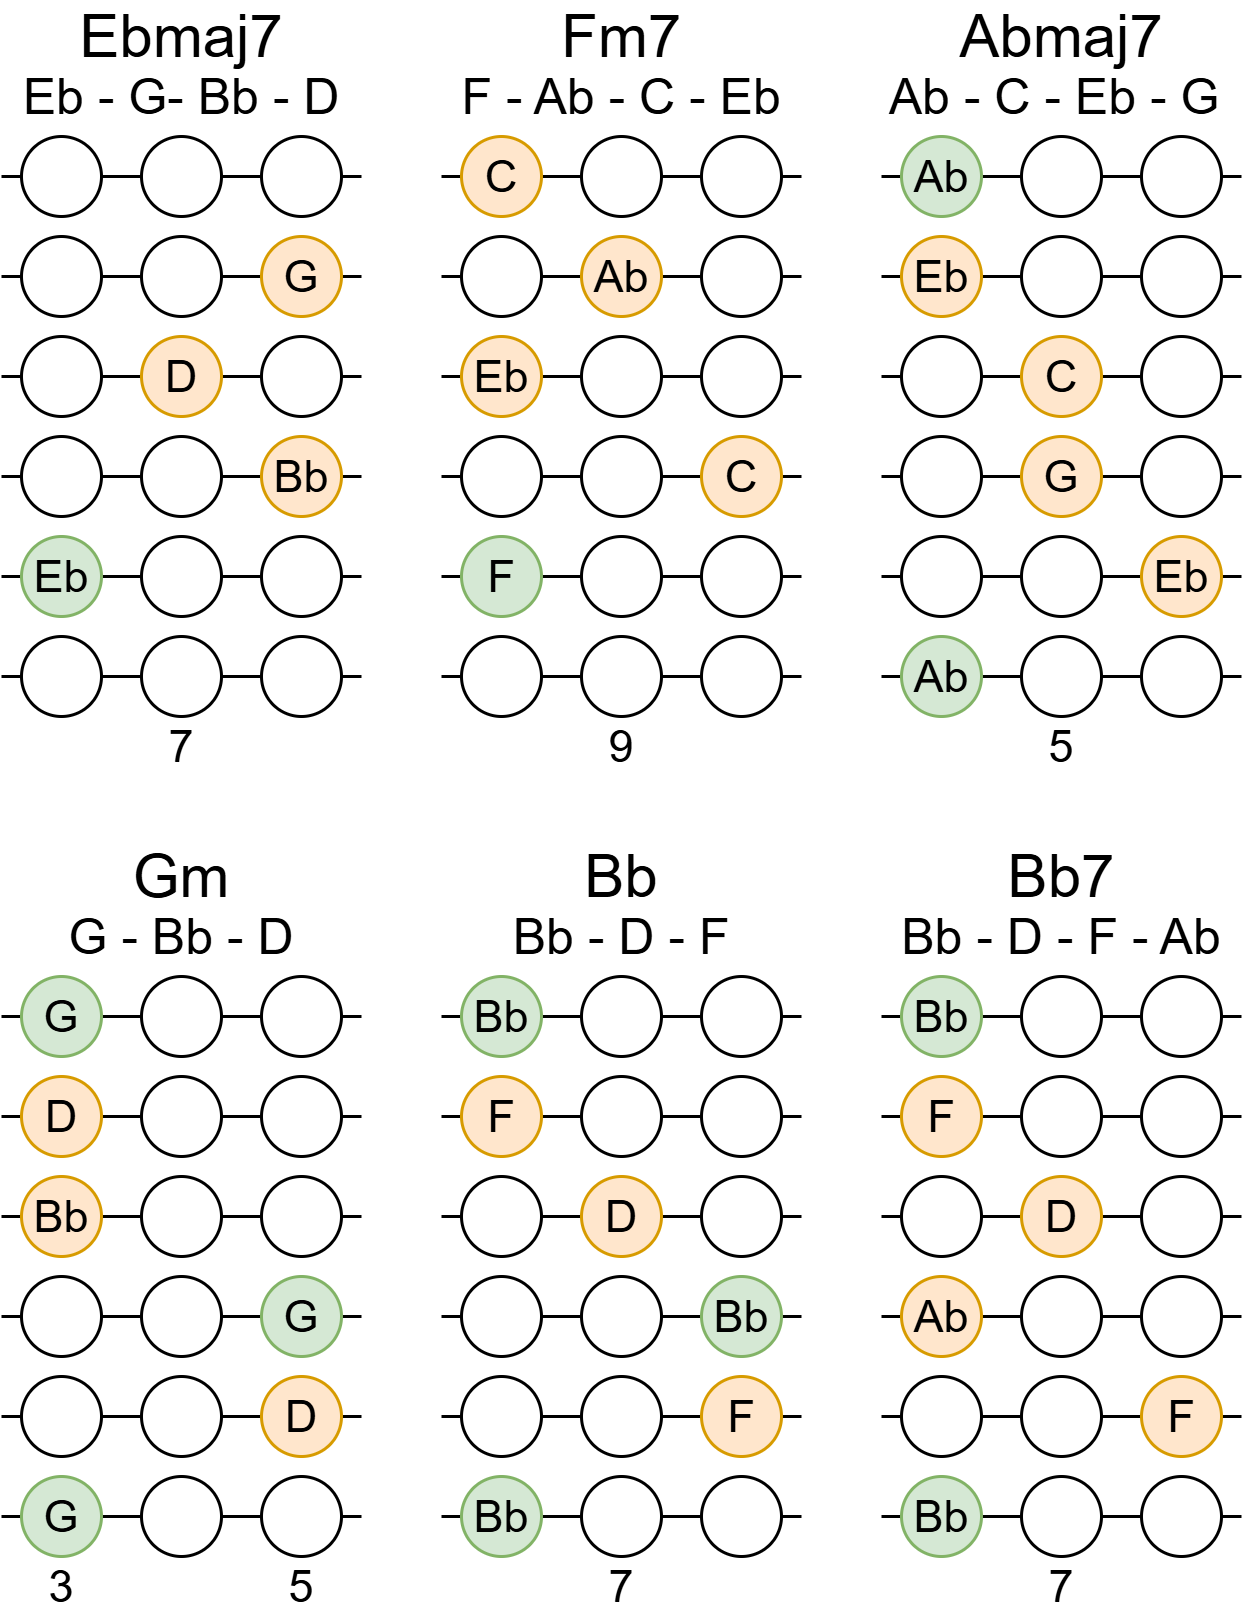
\includegraphics[width=0.55\textwidth]{../../Images/ChordsInValerieAmyWinehouse.png}
	\caption{Chords used in "Valerie- Amy Winehouse"}
	\label{fig:guitar_chords_valerie_amy_winehouse}
\end{figure}

\begin{song}[align-chords=l]{title={Valerie - Amy Winehouse (first verse + chorus)}, music={Amy Winehouse}}
	\begin{verse}
		^{Ebmaj7}Well, sometimes I go out by myself, and I look across the ^{Fm7}water \\
		And I ^{Ebmaj7}think of all the things, what you're doin', and in my head, I paint a ^{Fm7}picture \\
	\end{verse}
	\begin{chorus}
		^{Abmaj7}Since I've come on home, well, ^{Gm}my body's been a mess \\
		And I've ^{Abmaj7}missed your ginger hair, and ^{Gm}the way you like to dress \\
		^{Abmaj7}Won't you come on over? \\
		^{Gm}Stop makin' a fool out of ^{Bb}me \\
		^{Bb7}Why don't you come on over, Val^{Ebmaj7}erie? \\
		Val^{Fm7}erie, yeah \\
		Val^{Ebmaj7}erie, Val^{Fm7}erie \\
	\end{chorus}
\end{song}

\newpage

A song that has all the 4 different 7th chords that occur in the diatonic scale, is "Fly Me To The Moon" by "Frank Sinatra". The chord diagrams are shown in \autoref{fig:guitar_chords_fly_me_to_the_moon_frank_sinatra}.

Note that there are two versions of the \writechord{Am7} chord. The closed/barre version is only used for the first chord of the songs. After that, the open shape is used. The reason for this is the chords that follow and/or precede the \writechord{Am7} chord. The first \writechord{Am7} is followed by a barre version of the \writechord{Dm7} chords. Both are on the position of the 5th fret. Playing the barre versions of these chords have a little bit of a brighter sounds due to the common high A note on the first E string. You could of course play the open version of \writechord{Am7} and then either play the barre or the open version of the \writechord{Dm7} chord. Neither is correct or wrong. It's a matter of what you think sounds the best. For the rest of the verse the open version of the \writechord{Am7} is played. Also here it is because the surrounding chords are closer to the sound of open \writechord{Am7} chord than the barre chord. A second reason is because the chords are played closer to each other, resulting in less hand movement. But feel free to experiment with which version/voicing of the chords you think sound best.

\begin{figure}[h]
	\centering
	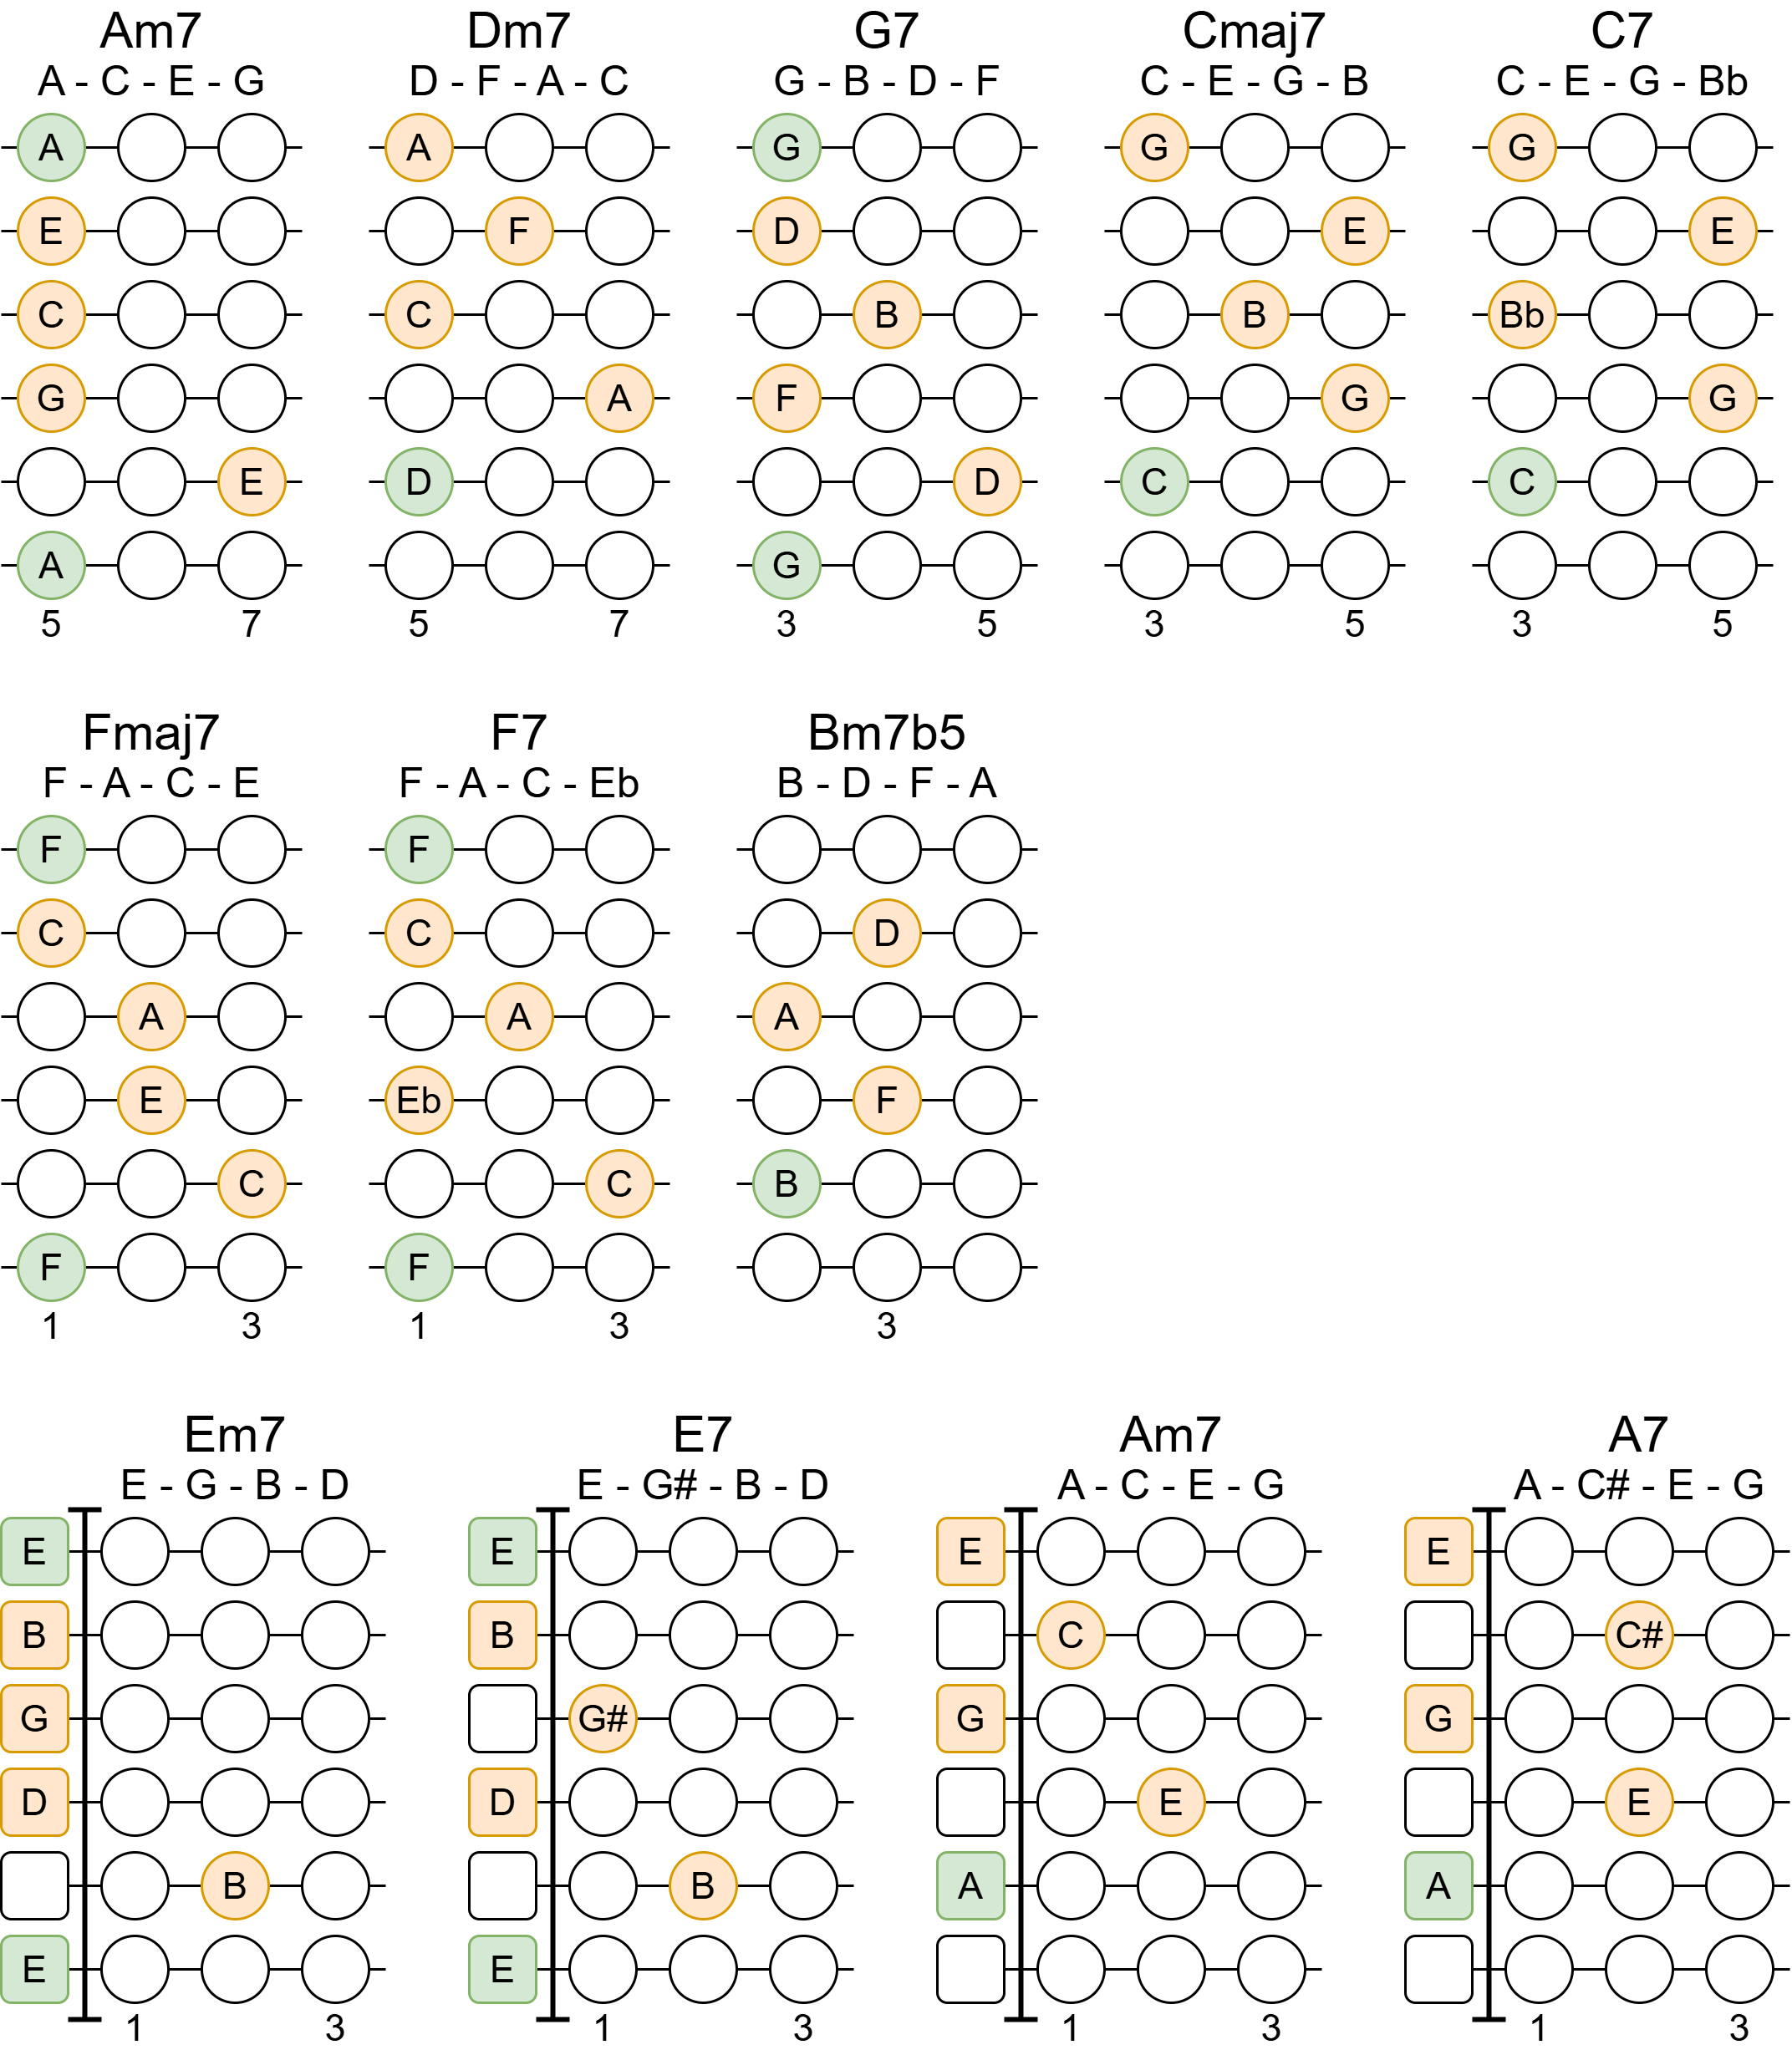
\includegraphics[width=0.65\textwidth]{../../Images/ChordsInFlyMeToTheMoonFrankSinatra.png}
	\caption{Chords used in "Fly Me To The Moon - Frank Sinatra"}
	\label{fig:guitar_chords_fly_me_to_the_moon_frank_sinatra}
\end{figure}

\begin{song}[align-chords=l]{title={Fly Me To The Moon - Frank Sinatra (first verse)}, music={Frank Sinatra}}
	\begin{verse}
		^{Am7}Fly me to the ^{Dm7}moon \\
		Let me ^{G7}play among the ^{Cmaj7}stars ^{C7}  \\
		And ^{Fmaj7}let me see what ^{Bm7b5}spring is like \\
		On a-^{E7}Jupiter and ^{Am7}Mars ^{A7}  \\
		^{Dm7}In other words, ^{G7} hold my ^{Cmaj7}hand ^{F7} ^{Em7} ^{A7}  \\
		^{Dm7}In other words, ^{G7} baby, ^{Cmaj7}kiss me ^{Bm7b5} ^{E7} \\
	\end{verse}
\end{song}

\newpage

\section{Suspended (sus) chords}

A suspended chord replaces the 3rd degree of the chord with either a major 2nd (sus2) or a perfect 4th (sus4).

This results in a chord that is neither major, nor minor. Note that both the major and minor scales have a major 2nd and a perfect 4th. Suspended chords are often played as short alterations to make the music sound a bit more lively while keeping the same root.

The tables below show the sus2 and sus4 structure.

\begin{table}[h]
	\begin{minipage}{0.45\textwidth}
		\centering
		\begin{NiceTabular}{*{16}{P{0.05mm}}}
			\Block{}{} & \Block{1-2}{\large{W}} & & \Block{1-2}{\large{W}} & & \Block{1-2}{\large{H}} & & \Block{1-2}{\large{W}} & & \Block{1-2}{\large{W}} & & \Block{1-2}{\large{W}} & & \Block{1-2}{\large{H}} & & \Block{}{} \\
			\Block[fill=ColorRootNote]{1-2}{1} & & \Block[fill=ColorOtherNote]{1-2}{2} & & \Block{1-2}{3} & & \Block{1-2}{4} & & \Block[fill=ColorOtherNote]{1-2}{5} & & \Block{1-2}{6} & & \Block{1-2}{7} & & \Block{1-2}{8} &
		\end{NiceTabular}
		\caption{Building a sus2 chord from the major scale}
		\label{tab:guitar_sus2_chord_buildup_major_scale}
	\end{minipage}
	\hfill
	\begin{minipage}{0.45\textwidth}
		\centering
		\begin{NiceTabular}{*{16}{P{0.05mm}}}
			\Block{}{} & \Block{1-2}{\large{W}} & & \Block{1-2}{\large{W}} & & \Block{1-2}{\large{H}} & & \Block{1-2}{\large{W}} & & \Block{1-2}{\large{W}} & & \Block{1-2}{\large{W}} & & \Block{1-2}{\large{H}} & & \Block{}{} \\
			\Block[fill=ColorRootNote]{1-2}{1} & & \Block{1-2}{2} & & \Block{1-2}{3} & & \Block[fill=ColorOtherNote]{1-2}{4} & & \Block[fill=ColorOtherNote]{1-2}{5} & & \Block{1-2}{6} & & \Block{1-2}{7} & & \Block{1-2}{8} &
		\end{NiceTabular}
		\caption{Building a sus4 chord from the major scale}
		\label{tab:guitar_sus4_chord_buildup_major_scale}
	\end{minipage}
	
	\begin{minipage}{0.45\textwidth}
		\centering
		\begin{NiceTabular}{*{16}{P{0.05mm}}}
			\Block{}{} & \Block{1-2}{\large{W}} & & \Block{1-2}{\large{H}} & & \Block{1-2}{\large{W}} & & \Block{1-2}{\large{W}} & & \Block{1-2}{\large{H}} & & \Block{1-2}{\large{W}} & & \Block{1-2}{\large{W}} & & \Block{}{} \\
			\Block[fill=ColorRootNote]{1-2}{1} & & \Block[fill=ColorOtherNote]{1-2}{2} & & \Block{1-2}{3$\flat$} & & \Block{1-2}{4} & & \Block[fill=ColorOtherNote]{1-2}{5} & & \Block{1-2}{6$\flat$} & & \Block{1-2}{7$\flat$} & & \Block{1-2}{8} &
		\end{NiceTabular}
		\caption{Building a sus2 chord from the minor scale}
		\label{tab:guitar_sus2_chord_buildup_minor_scale}
	\end{minipage}
	\hfill
	\begin{minipage}{0.45\textwidth}
		\centering
		\begin{NiceTabular}{*{16}{P{0.05mm}}}
			\Block{}{} & \Block{1-2}{\large{W}} & & \Block{1-2}{\large{H}} & & \Block{1-2}{\large{W}} & & \Block{1-2}{\large{W}} & & \Block{1-2}{\large{H}} & & \Block{1-2}{\large{W}} & & \Block{1-2}{\large{W}} & & \Block{}{} \\
			\Block[fill=ColorRootNote]{1-2}{1} & & \Block{1-2}{2} & & \Block{1-2}{3$\flat$} & & \Block[fill=ColorOtherNote]{1-2}{4} & & \Block[fill=ColorOtherNote]{1-2}{5} & & \Block{1-2}{6$\flat$} & & \Block{1-2}{7$\flat$} & & \Block{1-2}{8} &
		\end{NiceTabular}
		\caption{Building a sus4 chord from the minor scale}
		\label{tab:guitar_sus4_chord_buildup_minor_scale}
	\end{minipage}
\end{table}

\subsection{Notation}

Sus chords are noted as follows (taking C as the base chord):

\begin{itemize}
	\item Csus2
	\item Csus4
\end{itemize}

\subsection{Inversions of sus chords}

An interesting property of suspended chords is that inverting them results in a different sus chord.

In the following diagrams, the numbers from which, and to which, arrows are drawn, show the scale degree. The numbers on the arrows indicate how many half steps are in the interval between them.

\begin{tikzcd}
	degree \ar[r,"interval"] & degree \ar[r,"interval"] & degree  \ar[ll,bend left,dashed,"interval"]
\end{tikzcd}

\autoref{tab:guitar_sus_inversions} show the inversions of sus2 and sus4 chords.

Here also the term \textit{quartal chord} is mentioned. This is a chord that is build by stacking perfect 4th intervals.

\begin{table}[h]
	\centering
	\begin{NiceTabular}{P{4.5cm}|P{4.5cm}|P{4.5cm}}
		\Block{1-3}{\textit{sus2}} & & \\ 
		\hline
		Root & First inversion & Second inversion \\
		\textbf{sus2} & Quartal chord with 2 as root & \textbf{sus4} with 5 as root \\
		\hline
		{
			\begin{tikzcd}
				1 \ar[r,"2"] & 2 \ar[r,"5"] & 5 \ar[ll,bend left,dashed,"5"]
			\end{tikzcd}
		}
	 	& {
	 		\begin{tikzcd}
	 			2 \ar[r,"5"] & 5 \ar[r,"5"] & 1 \ar[ll,bend left,dashed,"2"]
	 		\end{tikzcd}
 		} & {
 			\begin{tikzcd}
	 			5 \ar[r,"5"] & 1 \ar[r,"2"] & 2 \ar[ll,bend left,dashed,"5"]
 			\end{tikzcd}} \\
		\hline
		\Block{1-3}{} & & \\
		\Block{1-3}{\textit{sus4}} & & \\
		\hline
		Root & First inversion & Second inversion \\
		\textbf{sus4} & \textbf{sus2} with 4 as root & Quartal chord with 5 as root \\
		\hline
		{
			\begin{tikzcd}
				1 \ar[r,"5"] & 4 \ar[r,"2"] & 5 \ar[ll,bend left,dashed,"5"]
			\end{tikzcd}
		}
		& {
			\begin{tikzcd}
				4 \ar[r,"2"] & 5 \ar[r,"5"] & 1 \ar[ll,bend left,dashed,"5"]
			\end{tikzcd}
		} & {
			\begin{tikzcd}
				5 \ar[r,"5"] & 1 \ar[r,"5"] & 4 \ar[ll,bend left,dashed,"2"]
		\end{tikzcd}} \\
	\end{NiceTabular}
	\caption{Intervals of sus4 chord inversions}
	\label{tab:guitar_sus_inversions}
\end{table}

\newpage

\subsection{Examples}

In the song "SummerOf'69" by "Bryan Adams" the sus2 and sus4 chords on the A and D chords are used at the end of the choruses, and in the last verse.

\begin{figure}[h]
	\centering
	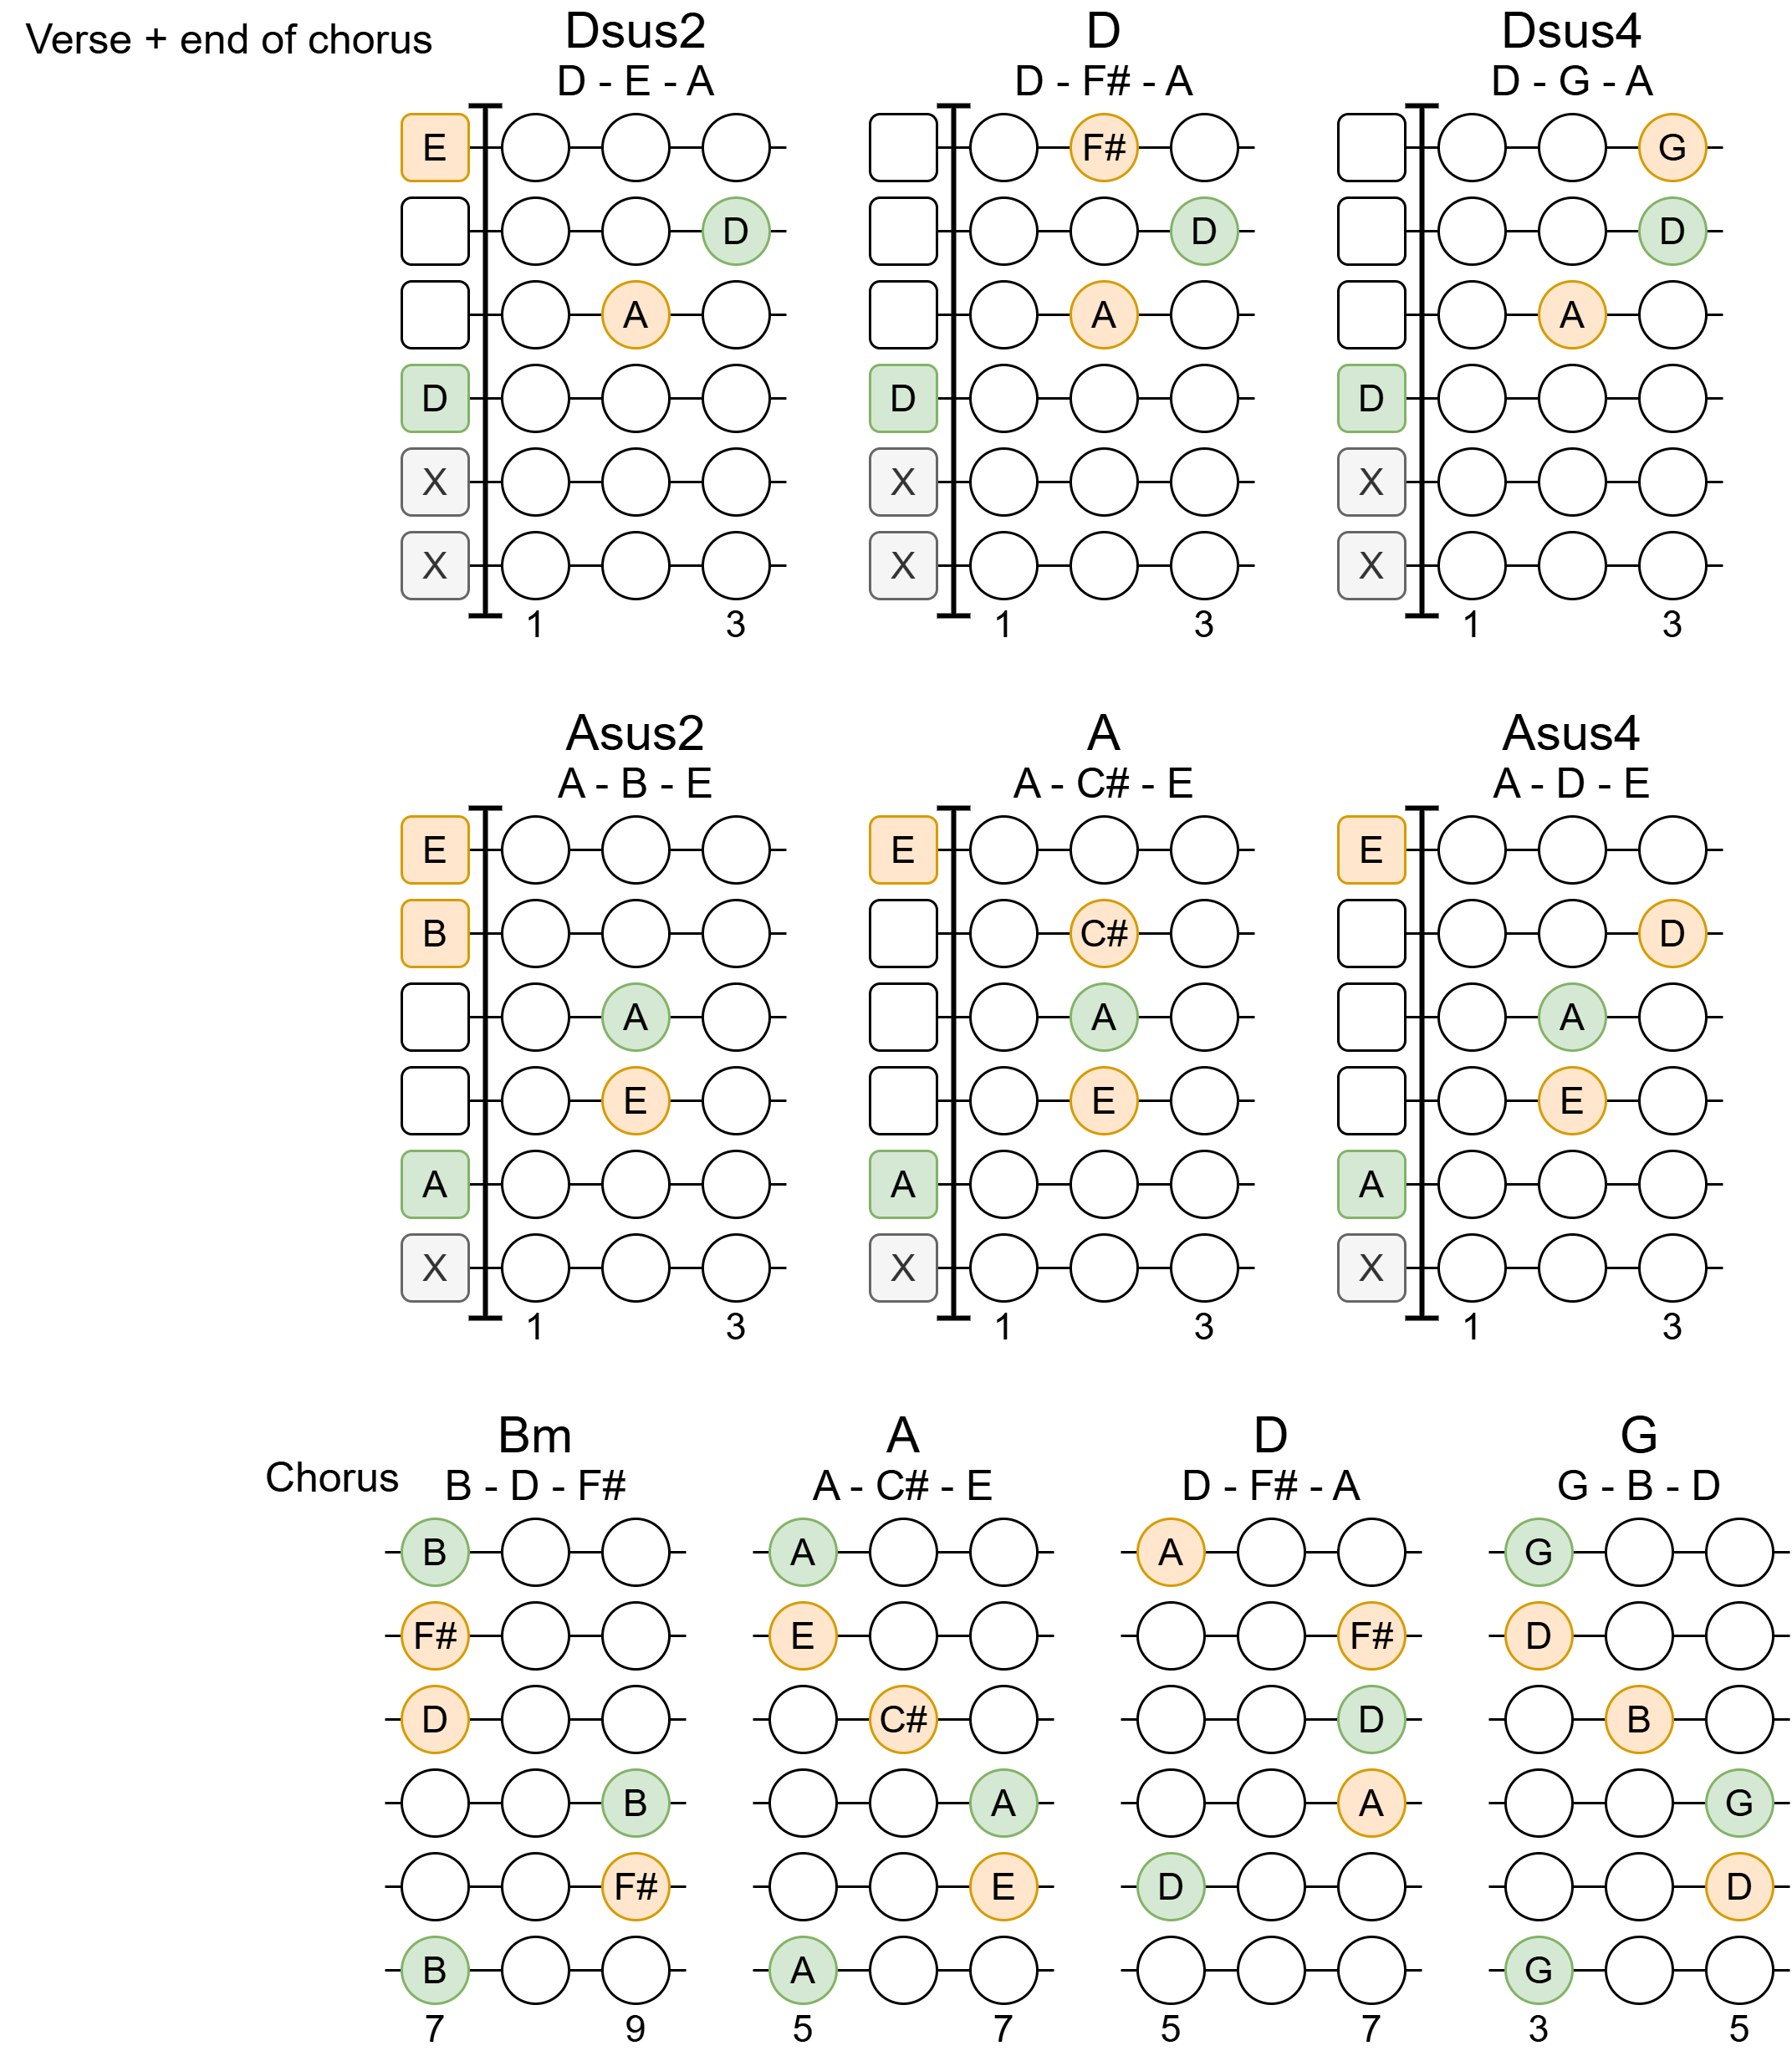
\includegraphics[width=0.65\textwidth]{../../Images/ChordsInSummerOf69BryanAdams.png}
	\caption{Chords used in "SummerOf'69 - Bryan Adams"}
	\label{fig:guitar_chords_summer_of_69_bryan_adams}
\end{figure}

\begin{song}[align-chords=l]{title={SummerOf'69 - Bryan Adams (last verse + chorus)}, music={Bryan Adams}}
	\begin{verse}
		^{Dsus2} ^{D}And now^{Dsus4} the times^{D} are^{Dsus2} chan^{D}gin' {} \\
		^{Asus2} Look^{A} at every^{Asus4}thing that's come^{A} and ^{Asus2}gone^{A} {} \\
		^{Dsus2} ^{D}Some^{Dsus4}times, when^{D} I play that old ^{Dsus2}six-^{D}string {} \\
		^{Asus2} Think^{A} about you, ^{Asus4}wonder what^{A} went ^{Asus2}wrong^{A} \\
	\end{verse}
	\begin{chorus}
		^{Bm} Standin' on your ^{A}mama's porch, ^{D} You told me that it'd ^{G}last forever \\
		^{Bm} Oh, and when you ^{A}held my hand, ^{D} I knew that it was ^{G}now or never \\
		^{Bm} Those were the ^{A}best days of my life \\
		^{Dsus2} ^{D} ^{Dsus4} ^{D} ^{Dsus2} Oh^{D}, yeah, \\
		^{Asus2} ^{A} ^{Asus4} ^{A}back in the ^{Asus2}summer ^{A}of ^{Dsus2}sixty ^{D}nine, ^{Dsus4} ^{D} ^{Dsus2} ^{D} \\
	\end{chorus}
\end{song}

\newpage

Suspended chords can also be used in a melody of course. The song "Breath" from "Rioghan" uses this (\autoref{fig:guitar_breath_rioghan_intro}).

\begin{figure}[h]
	\centering
	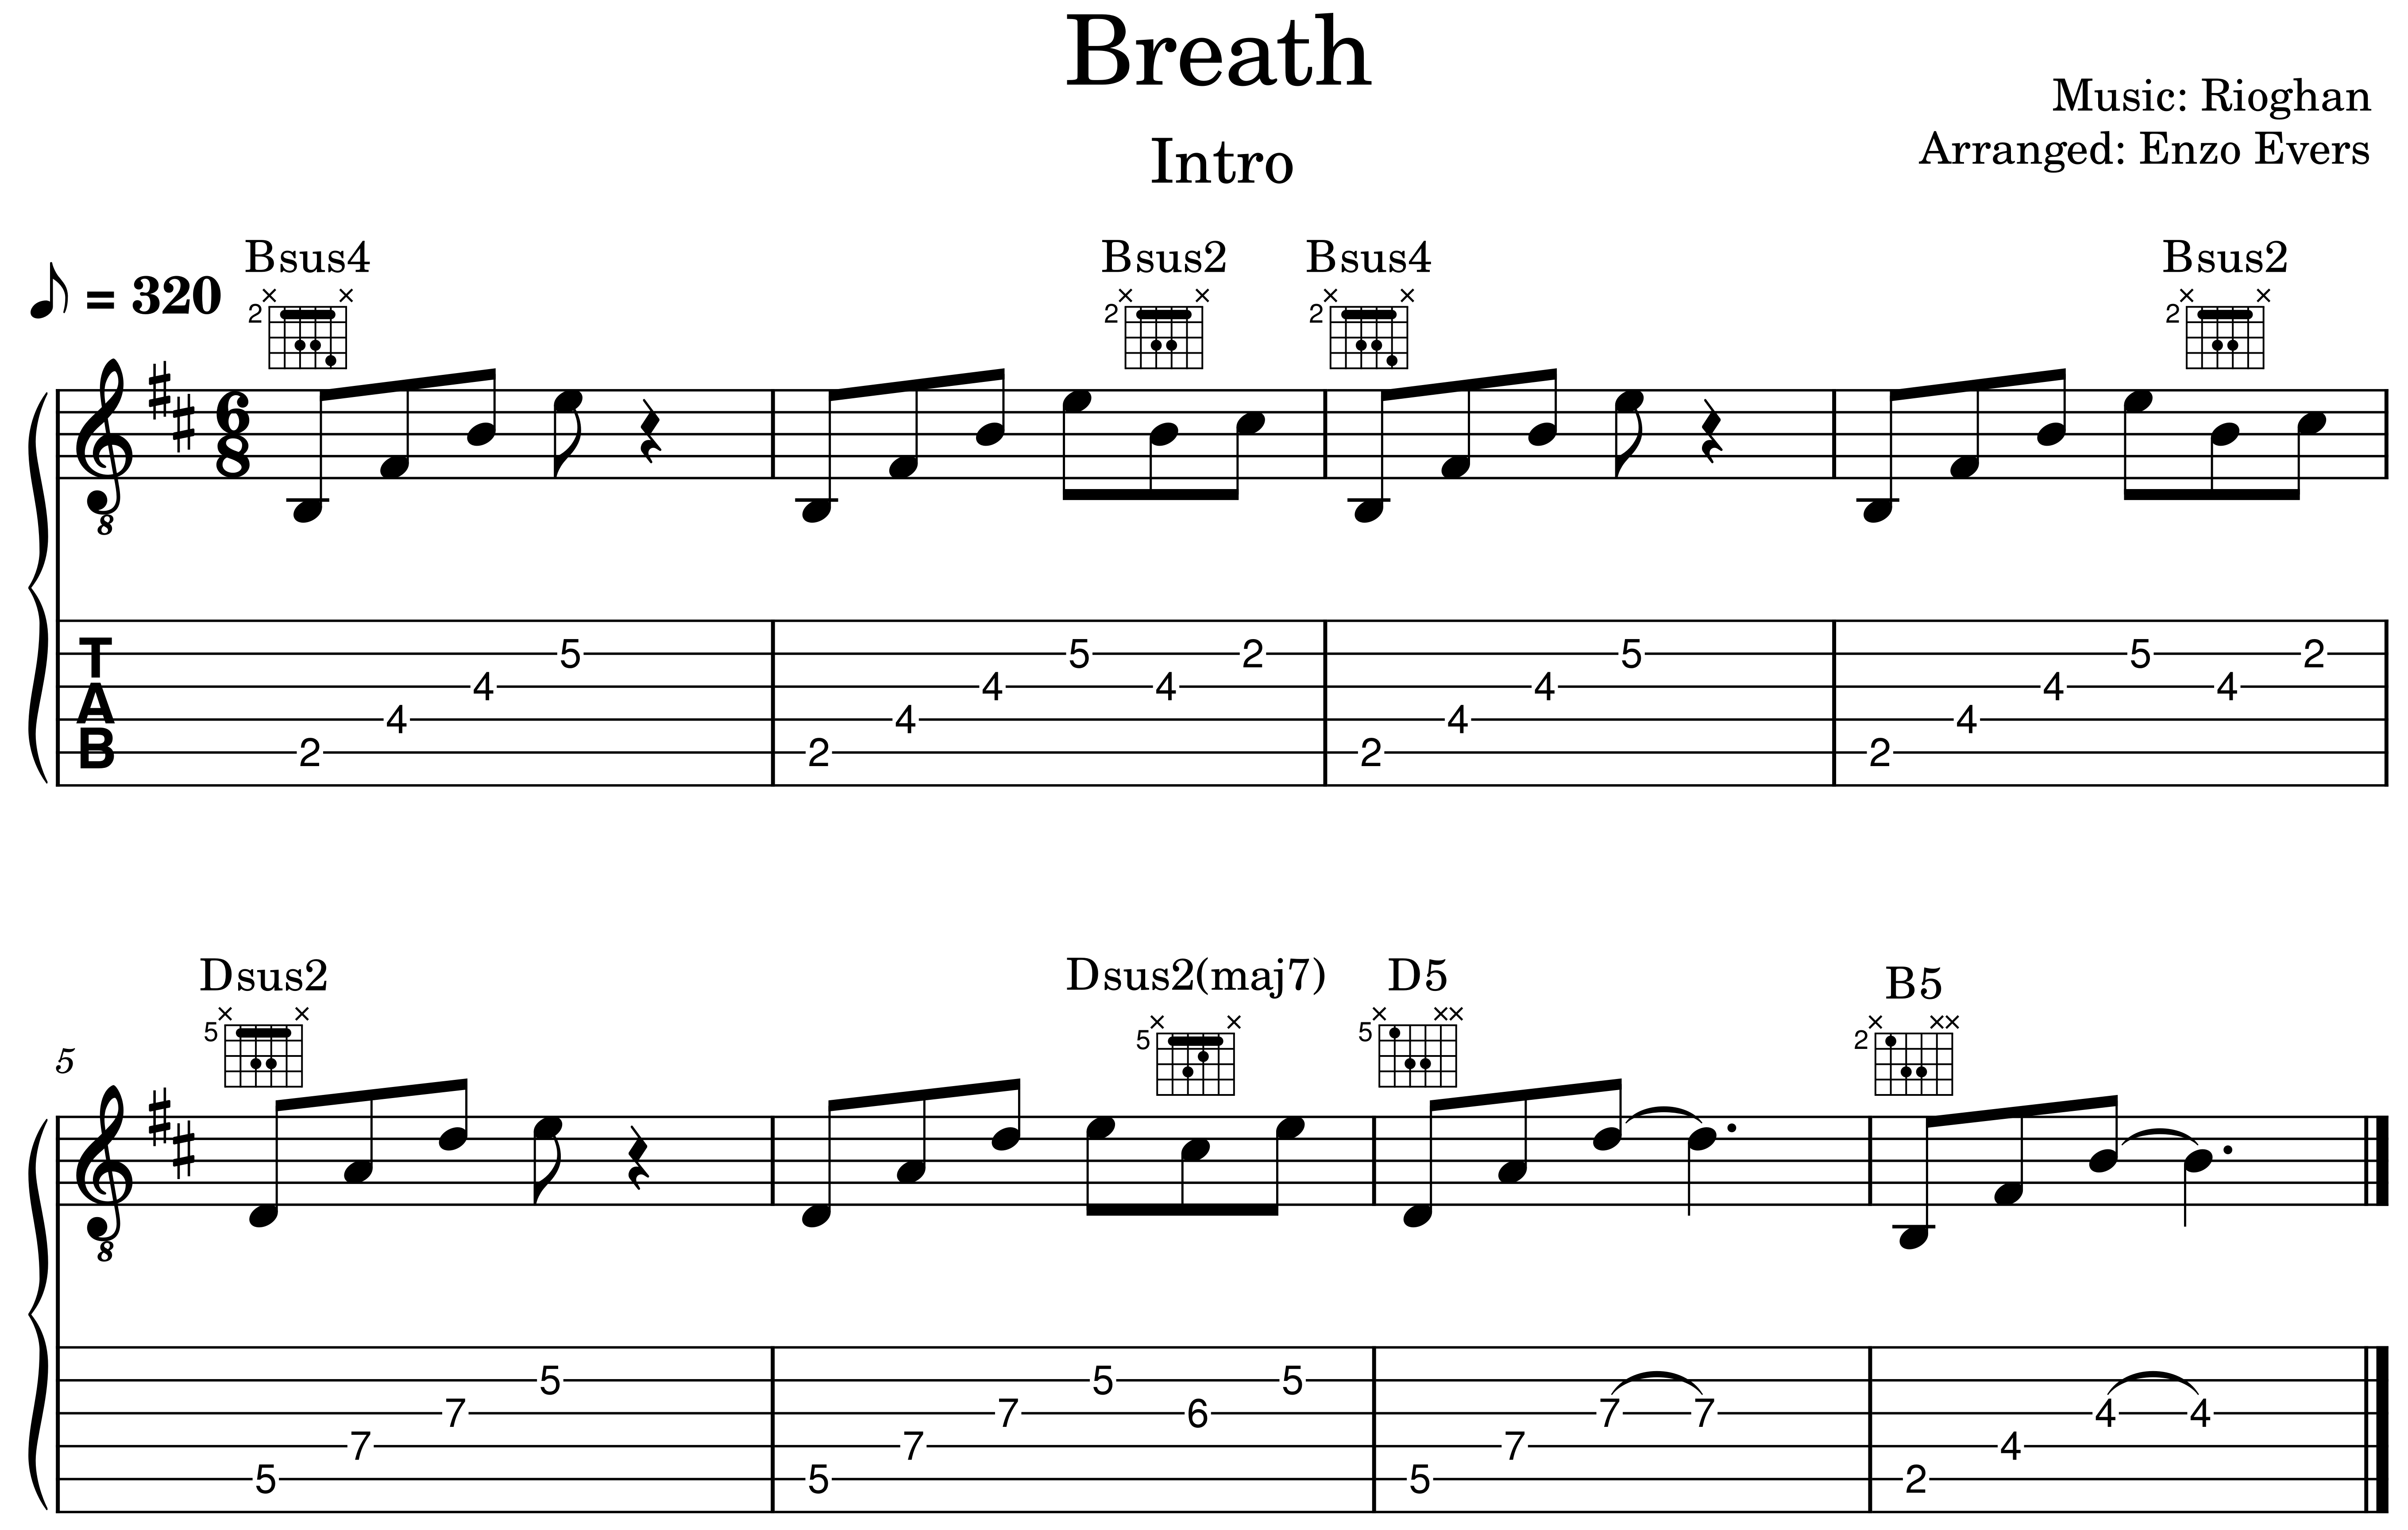
\includegraphics[width=\textwidth]{../../MuseScore/Guitar/GuitarBreathRioghanIntro.png}
	\caption{Intro of "Breath" by "Rioghan"}
	\label{fig:guitar_breath_rioghan_intro}
\end{figure}


% Summer of 69 - Bryan Adams
% Breath - Rioghan
% Cold as ice - Foreigner
% Wonderboy - tenacious D
% Inversions

\newpage

\section{Extended \& Add chords}
TODO
